\section{A Discrete Model of Powder Particles}\label{sec:particle-model}

\begin{itemize}
    \item Particles, Coordinate System
    \item Node Types
    \item Multi-Scale Considerations, Matrix
\end{itemize}

Continuous description of the particle surface geometry is only possible for nearly ideal geometries.
For complicated geometries a discretized approach is feasible.
For the current work, the concept of a node shall be introduced.
A node is here considered as a discrete point of the particle surface connected with its neighbors by straight lines.
The spline of those lines is defining the surface of the particle.

The location of each node in space is defined by a tuple of polar coordinates $(\Angle, \Radius)$, where $\Angle$ is the angle coordinate and $\Radius$ the radius resp.~distance from origin.
The origin of the polar coordinates is distinct for each particle and is considered as the center of the particle, although it is generally not identical with the barycenter of the particle.
But the center of the particle is used as an anchor for defining a particles postions in space.
With this concept the particle can be moved in space without translating the surface node coordinates and the description of node evolution is simplified, since only the local geometry must be regarded.
Particle movement occurs due to diffusional fluxes in the grain boundaries, which is macroscopically observed as shrinkage.
The location of a particle is defined by the cartesian coordinates of its center $\X$ and $\Y$, as well as a rotation angle $\RotationAngle$ with the center as pole.
The rotation angle always counts from the $\X$-axis on in mathematical direction.
The rotation angle also defines the origin axis of the particles local coordinate system.
See \autoref{fig:model_development/particle_coordinates} for illustration on this.

\begin{figure}
    \centering
    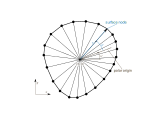
\includegraphics{img/model_development/particle_coordinates}
    \caption{Position of a Particle and Its Local Coordinate System}
    \label{fig:model_development/particle_coordinates}
\end{figure}

In regard of sintering processes, the contact properties of multiple particles are investigated.
The common interface of two particles in contact is commonly called a sinter neck.
It consists of a grain boundary bounded by triple points of the grain boundary and the two adjacent free surfaces.
\autoref{fig:model_development/two_particle_contact} shows such a contact of two particles.
Until here, three types of nodes can be identified:
\begin{description}
    \item[Surface Nodes] forming the free surface of a particle in contact to atmosphere or vacuum (black).
    \item[Grain Boundary Nodes] forming the grain boundary in a particle contact (dark blue).
    \item[Neck Nodes] representing the triple point between grain boundary and two surfaces (dark red).
\end{description}
Details on the conditions at those nodes are given in the following sections.
The particles are named as \emph{parent} and \emph{child}, since every particle contact shall be regarded in a hierarchical manner.
The reason for that lies in the graph description of contact topology described below.
The contact is characterized by the length and the direction of the line connecting the involved particles' centers.
Since every particle has its own polar coordinate system, measures of contact and coordinates of nodes involved can be regarded in either the parent's or the child's coordinate system.
The coordinate system used shall be denoted hereinafter by ${}^{|\square}$ superscripts where necessary as done in the figure.
So the direction ange of the contact is $\Angle_\Contact^{|\Parent}$ or $\Angle_\Contact^{|\Child}$ in means of the parent's or the child's coordinate system, respectively.
The coordinates of one neck node are shown in the figure as $(\Angle^{|\Parent}, \Radius^{|\Parent})$ and $(\Angle^{|\Child}, \Radius^{|\Child})$.
Note, that both tuples represent the same point in space.

\begin{figure}
    \centering
    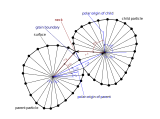
\includegraphics{img/model_development/two_particle_contact}
    \caption{Contact of Two Particles with Respective Properties}
    \label{fig:model_development/two_particle_contact}
\end{figure}

The contact topology of multiple particles can be described as a graph, where the vertices correspond to particles and the edges correspond to contact relations between the particles.
The undirected graph structure of a particle contact is shown in \autoref{fig:model_development/particle_graph}.
The indices of the vertices are at this point arbitrary, but are reused in the same way in the following.

For simulation purposes, the introduction of a hierarchy in the particle contacts is feasible to introduce a specific order for equation construction.
More specifically the particle contacts shall be described as a~\gls{DAG}.
Such a graph can always be constructed from a given undirected graph by performing a \gls{BFGS} starting at the desired root vertex and dropping all edges pointing back to the parent.
An example of such a structure in shown in \autoref{fig:model_development/particle_graph_dag}.
The particle labeled with index 0 is the \emph{root} of the graph, the only vertex that has no incoming edges.
In general, the root of the particle graph can be chosen arbitrarily, but for efficiency reasons, it should be a particle which leads to a graph as flat as possible.
The root particle has a fixed position in space and therefore acts as origin for all coordinate systems used throughout the calculations.
There may be cases, where the particle graph has rooted tree structure, which simplifies the problem significantly, since then all particles are able to move freely.
Edges like the red one in the figure break the tree structure.
Note, that they do not form cycles in the~\gls{DAG} in the meaning of graph theory, since the edges are directed.
But in terms of the underlying undirected graph they are anyway cycles.
To avoid ambiguities, the term ring contact shall be used here instead.
Ring contacts introduce additional constraints to the particle movement, since each particle in the ring influences the movement of the others.
The edges closing a ring are named correspondingly as \glspl{RCE}.

\begin{figure}
    \centering
    \includegraphics{img/model_development/particle_graph}
    \caption{Undirected Particle Graph Representing Contact Conditions}
    \label{fig:model_development/particle_graph}
\end{figure}

\begin{figure}
    \centering
    \includegraphics{img/model_development/particle_graph_dag}
    \caption{Directed Acyclic Graph Structure of Particle Contacts Rooted at Vertex 0}
    \label{fig:model_development/particle_graph_dag}
\end{figure}

\Glspl{RCE} are discovered during a~\gls{BFGS} when a vertex is encountered that was already marked as visited.
To be able to construct geometric constraints on particle movement, a ring path must be defined.
A ring path is a path following the cycle in the undirected graph, the currently regarded ring corresponds to.
It is generally not unique, but this is also not necessary.
To find a ring path, a~\gls{DFGS} is performed on the undirected particle graph with the ring closing edge removed.
The removed edge is afterwards appended to the path to close the ring.
The procedure is illustrated in \autoref{fig:model_development/particle_graph_ring_search}.

\begin{figure}
    \centering
    \includegraphics{img/model_development/particle_graph_ring_search}
    \caption{Ring Path Search Using a Depth-First Graph Search}
    \label{fig:model_development/particle_graph_ring_search}
\end{figure}


